\documentclass[tikz]{standalone}
\usepackage{circuitikz}
\begin{document}


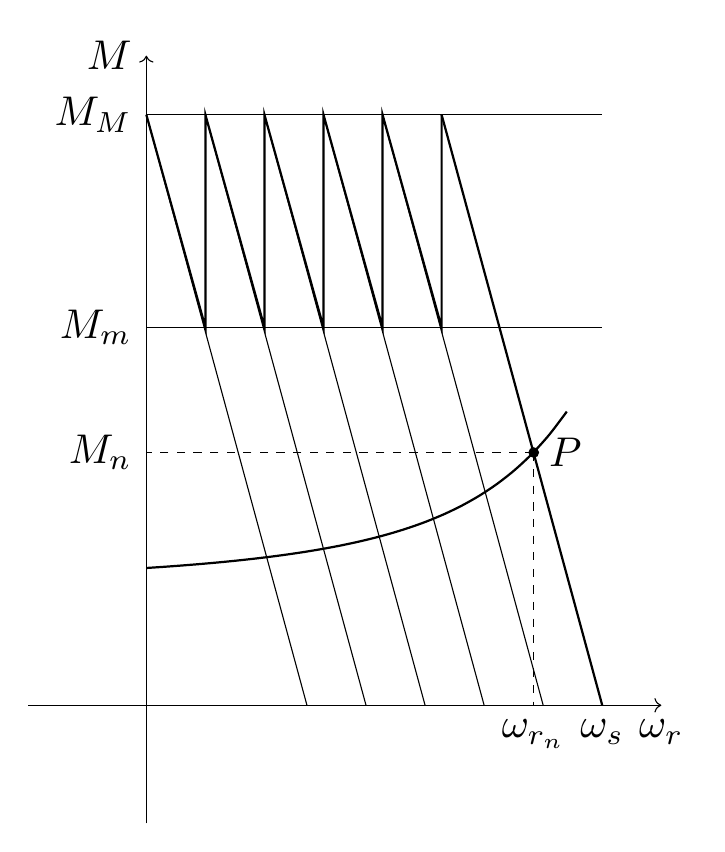
\begin{tikzpicture}[scale=1.5, transform shape]
  \draw[->] (-0.86,0) -- (4.5,0) node[below] {$\omega_r$};
  \draw[->] (0.14,-1) -- (0.14,5.5) node[left] {$M$};
  \draw[ black] (0.14,5) node[left]{$M_{M}$} ;
  \draw (4,0) node[below] {$\omega_s$};
  %\draw[ black] (1.2,5) -- (4,0);
  %\draw[ black] (2.05,5) -- (4,0);
  \draw[thick, black] (2.64,5) -- (4,0);
  \draw[ black] (2.14,5) -- (3.5,0);
  \draw[ black] (1.64,5) -- (3,0);
  \draw[ black] (1.14,5) -- (2.5,0);
  \draw[ black] (0.64,5) -- (2,0);
  \draw[ black] (0.14,5) -- (1.5,0);
  
  \draw [black] (0.14,5) -- (4,5);
  \draw [black] (0.14,3.2) node[left]{$M_{m}$} -- (4,3.2);
 
  \draw[thick, black] (0.14,5) -- (0.64,3.2) -- (0.64,5) -- (0.64,3.2) -- (0.64,5) -- (1.14,3.2) 
  --(1.14,5) -- (1.64,3.2) -- (1.64,5) -- (2.14,3.2) -- (2.14,5) -- (2.64,3.2) -- (2.64,5);

  
 \draw[thick, black, domain=0.14:3.7, smooth] plot (\x, {1+4/(1 + (\x - 5)^2)});                  

 \draw[thick, black,fill=black] (3.42,2.14) circle (1pt) node[right] {$P$};
 \draw[dashed] (3.42,2.14) -- (3.42,0) node[below]{$\omega_{r_n}$};
  \draw[dashed] (3.42,2.14) -- (0.14,2.14) node[left]{$M_n$};
\end{tikzpicture}



\end{document}
